\documentclass[conference,a4paper]{IEEEtran}
% IEEE conference format (IEEEtran.cls is included in this folder).

\usepackage{amsmath,amssymb}
\usepackage{graphicx}
\usepackage{booktabs}
\usepackage{cite}
\usepackage{url}
\usepackage[hidelinks]{hyperref}

\graphicspath{{../figures/}}

\newcommand{\w}{\mathbf{w}}
\newcommand{\x}{\mathbf{x}}
\newcommand{\Sig}{\boldsymbol{\Sigma}}

\begin{document}

\title{Correlated Uncertainty, Not Drift: What a Kalman-Filter Learner Explains
About Retrospective Revaluation That Rescorla--Wagner Cannot}

\author{\IEEEauthorblockN{Solanki Viraj Rajeshbhai}
\IEEEauthorblockA{Roll No.\ 24110348\\
CG-501 Computation and Cognition, End-Term Project Report\\
Indian Institute of Technology Gandhinagar\\
Code: \url{https://github.com/Viraj-Solanki/CG-501}}}

\maketitle

%=====================================================================
\begin{abstract}
The Rescorla--Wagner (RW) rule explains cue competition, but it cannot change
the associative strength of an absent cue. It therefore predicts no backward
blocking or unovershadowing, although both are observed. A Kalman-filter learner
tracks a mean and a covariance over the cue weights and uses uncertainty-driven
learning rates. I implemented RW, the full Kalman learner, a Kalman learner without
cross-cue covariance, and an RW variant with within-compound associations. I
validated them against closed-form solutions and qualitatively reproduced a
published backward-blocking simulation. Only the full Kalman learner showed
backward blocking ($0.42$) and unovershadowing ($0.42$), in 20/20 reward-noise
seeds. Removing the off-diagonal covariance abolished both effects at all 100 noise
settings, while forward blocking survived. Process noise was \emph{not} required:
backward blocking was present with zero drift and depended non-monotonically on
drift. The responsible component is the correlated uncertainty between cues, not
uncertainty-driven learning rates as such. The within-compound model also produced
both effects, but with a different dependence on trial order.
\end{abstract}

\begin{IEEEkeywords}
classical conditioning, Rescorla--Wagner model, Kalman filter, backward blocking,
retrospective revaluation, Bayesian learning
\end{IEEEkeywords}

%=====================================================================
\section{Introduction}
%=====================================================================
\subsection{Background and Rationale}
In classical conditioning an animal learns which cues predict an outcome. The
Rescorla--Wagner model \cite{rescorla1972} formalises this as error-correcting
learning: each present cue $i$ changes its weight $w_i$ in proportion to a
prediction error shared by all present cues. Because the error is shared, cues
compete. A cue trained first \emph{blocks} learning about a cue added later
(forward blocking), and two cues trained together \emph{overshadow} each other.

RW has a structural blind spot. A cue that is absent on a trial has $x_i = 0$,
so its weight cannot change. Yet in \emph{backward blocking}, training a compound
AB$+$ and then B$+$ alone reduces responding to the absent cue A
\cite{shanks1985}. In \emph{unovershadowing}, extinguishing A after AB$+$
\emph{increases} responding to B \cite{matzel1985}. Both are cases of
retrospective revaluation: learning about a cue that is not presented. They are a
clean test of what a learning rule represents beyond single point estimates.

Statistical inference offers an explanation. If the learner keeps a distribution
over the weights, AB$+$ trials tell it only that $w_A + w_B \approx 1$, so the two
weights become negatively correlated, and later evidence that B alone predicts
reward \emph{explains away} A \cite{dayan2001}. This project asks which part of
the Bayesian machinery is responsible.

\subsection{Review of Relevant Literature}
Sutton \cite{sutton1992} proposed that conditioning can be understood as Kalman
filtering, in which per-cue learning rates (``gains'') track uncertainty. To keep
the computation cheap he approximated the weight covariance by its diagonal.
Dayan \emph{et al.} \cite{dkm2000} used this framework to cast selective attention
in conditioning as statistically normative: the learning rate for cue $i$ is
$\sigma_i^2 x_i / (\sum_j \sigma_j^2 x_j + E)$, so prediction error is shared
among cues in proportion to their uncertainties. This is a Kalman filter with a
diagonal covariance, related to the Pearce--Hall idea that uncertain predictors
learn faster \cite{pearce1980}. Kakade and Dayan \cite{kakade2002} used
uncertainty-based learning rates to account for acquisition and extinction in
autoshaping. Dayan and Kakade \cite{dayan2001} showed that keeping the
\emph{full} covariance produces backward blocking as explaining away in weight
space. They also noted that Sutton's diagonal approximation ``prevents the system
from accounting for backward blocking''. Broader reviews of Bayesian associative
learning are given by Kruschke \cite{kruschke2008} and Gershman \cite{gershman2015}.

Non-Bayesian accounts exist too. Van Hamme and Wasserman \cite{vanhamme1994}
modified RW so that an absent but expected cue has a negative learning rate.
Wagner's SOP/AESOP framework gives a related within-compound explanation
\cite{wagner1989}. Empirically, backward blocking is robust in human causal
judgement \cite{shanks1985} but harder to obtain in animals. Miller and Matute
\cite{miller1996} argued that it depends on the target cue having low biological
significance.

\subsection{Hypotheses and Objectives}
\begin{enumerate}
\item[\textbf{H1}] A full-covariance Kalman learner will show backward blocking
and unovershadowing; RW will not. All models will show forward blocking and
overshadowing.
\item[\textbf{H2}] Removing the off-diagonal covariance will abolish backward
blocking and unovershadowing but leave forward blocking and overshadowing intact.
\item[\textbf{H3}] Larger process noise $\tau^2$ (expected volatility) will
speed acquisition and increase backward blocking, because it keeps uncertainty high.
\end{enumerate}
I tested these with a replication, a parameter sweep, an ablation and a competing model.

%=====================================================================
\section{Methods}
%=====================================================================
\subsection{Model Details}
Each trial presents a binary cue vector $\x_t$ (cues A, B, C) and a scalar
reward $r_t$. All models predict $\hat r_t = \x_t^\top \w$ and compute the prediction
error $\delta_t = r_t - \x_t^\top \w$.

\subsubsection{Rescorla--Wagner}
$w_i \leftarrow w_i + \alpha\, x_i\, \delta_t$, with $\alpha = 0.1$.

\subsubsection{Kalman Learner}
The learner assumes that the weights drift and that rewards are noisy:
\begin{equation}
\begin{aligned}
\w_t &= \w_{t-1} + \boldsymbol\eta_t, & \boldsymbol\eta_t &\sim\mathcal N(\mathbf 0,\tau^2\mathbf I),\\
r_t &= \x_t^\top\w_t + \varepsilon_t, & \varepsilon_t &\sim\mathcal N(0,\sigma^2).
\end{aligned}
\end{equation}
Its belief is $\w\sim\mathcal N(\hat\w,\Sig)$, with prior $\mathcal N(\mathbf 0,\sigma_0^2\mathbf I)$.
On each trial it applies the standard filter:
\begin{align}
\Sig^- &= \Sig + \tau^2\mathbf I, \label{eq:drift}\\
\mathbf k &= \frac{\Sig^-\x_t}{\x_t^\top\Sig^-\x_t + \sigma^2}, \label{eq:gain}\\
\hat\w &\leftarrow \hat\w + \mathbf k\,\delta_t, \label{eq:mean}\\
\Sig &\leftarrow \Sig^- - \mathbf k\,(\Sig^-\x_t)^\top. \label{eq:cov}
\end{align}
In words: drift makes uncertainty grow (\ref{eq:drift}); the Kalman gain is a
per-cue learning rate (\ref{eq:gain}); the mean moves by gain times error
(\ref{eq:mean}); and uncertainty shrinks after the outcome (\ref{eq:cov}).
The gain of an \emph{absent} cue $i$ is $k_i = \sum_j \Sigma^-_{ij}x_j / (\cdot)$. It
is non-zero whenever cue $i$ covaries with a present cue. This is the only route
by which an absent cue can change. Defaults: $\sigma^2 = 0.5$, $\tau^2 = 0.01$,
$\sigma_0^2 = 1$. Note that Dayan and Kakade \cite{dayan2001} use $\sigma^2$ for
drift and $\tau^2$ for observation noise, the reverse of my notation. They also
apply drift after the observation rather than before it; the two orders give the
same filter shifted by half a step.

\subsubsection{Ablation (Diagonal Kalman)}
After every update I set the off-diagonal entries of $\Sig$ to zero. This keeps
uncertainty-driven, competitively shared learning rates, and is the form used in
\cite{sutton1992} and \cite{dkm2000}. It removes all information about how the
cues covary.

\subsubsection{Alternative: RW With Within-Compound Associations}
Following the idea of \cite{vanhamme1994}, cue--cue associations $a_{ij}$ are
learned with a delta rule whenever cue $j$ is present:
$a_{ij}\leftarrow a_{ij} + 0.1\,x_j(x_i - a_{ij})$. An absent cue receives
activation $c_i = \min(1,\sum_j a_{ij}x_j)$ and learns with a negative rate:
$w_i \leftarrow w_i - 0.05\,c_i\,\delta_t$. This is my simplified implementation,
not the published equations.

\subsection{Implementation}
\subsubsection{Paradigms}
Each test schedule has a control matched in trial count and number of
reinforcements, using a third cue C (Table~\ref{tab:design}). Phases last 30
trials. An effect is the signed difference between test and control on the
critical cue at the end of training, so a positive value means the phenomenon is
present. Acquisition speed is the number of A$+$ trials until $w_A\geq0.9$.

\begin{table}[!t]
\centering\footnotesize
\setlength{\tabcolsep}{3pt}
\renewcommand{\arraystretch}{1.3}
\caption{Paradigms, Controls and Measures}
\label{tab:design}
\begin{tabular}{llll}
\toprule
Paradigm & Test & Control & Effect ($>0$: present)\\
\midrule
Fwd.\ blocking & A$+\to$AB$+$ & C$+\to$AB$+$ & $w_B^{\text{ctrl}} - w_B^{\text{test}}$\\
Overshadowing & AB$+$ & A$+$ & $w_A^{\text{ctrl}} - w_A^{\text{test}}$\\
Bwd.\ blocking (BB) & AB$+\to$B$+$ & AB$+\to$C$+$ & $w_A^{\text{ctrl}} - w_A^{\text{test}}$\\
Unovershad.\ (UO) & AB$+\to$A$-$ & AB$+\to$C$-$ & $w_B^{\text{test}} - w_B^{\text{ctrl}}$\\
\bottomrule
\end{tabular}
\end{table}

\subsubsection{Experiments}
(0)~Replication of all paradigms for the four models, plus a reproduction of the
exact-Kalman simulation in Fig.~2C--D of \cite{dayan2001}. (1)~A sweep over
$\tau^2\in\{0, 10^{-4},\dots,1\}$ (10 values) and $\sigma^2\in[0.01,10]$ (10
log-spaced values). (2)~Full versus diagonal covariance, including the effect of
AB$+$ phase length. (3)~Robustness: Gaussian noise (SD 0.2) added to rewards, 20
fixed seeds. Test and control receive the same noise sequence (common random
numbers). An earlier version used independent seeds and produced a spurious
``backward blocking'' of $0.037\pm0.049$ in RW, which is impossible for that
model. This was the motivation for the matched design.

\subsubsection{Validation}
Ten unit tests check known answers. (i)~RW converges to $r$ and matches
$w_t=r(1-(1-\alpha)^t)$ exactly. (ii)~With $\tau^2 = 0$, the Kalman mean and
covariance equal the closed-form Bayesian ridge posterior,
$\Sig=(\mathbf X^\top\mathbf X/\sigma^2+\mathbf I/\sigma_0^2)^{-1}$ and
$\hat\w=\Sig\mathbf X^\top\mathbf r/\sigma^2$, after \emph{every} trial
(tolerance $10^{-9}$). (iii)~With $\tau^2>0$, the steady-state predicted variance
for a single cue equals $(\tau^2+\sqrt{\tau^4+4\tau^2\sigma^2})/2$. (iv)~The
covariance stays symmetric and positive definite. (v)~Ablation and
model-reduction sanity checks. All tests pass.

The code uses plain NumPy and Matplotlib and is deterministic.
\texttt{python tests.py} runs the validation, and \texttt{python make\_figures.py}
regenerates every number and figure in this report; repeated runs give
byte-identical figures.

%=====================================================================
\section{Results}
%=====================================================================
\subsection{Does the Implementation Reproduce the Published Model?}
With the parameters reported in \cite{dayan2001} (drift SD 0.09, observation SD
0.35; I assumed $\Sig_0 = 0.09^2\,\mathbf I$, since theirs is not stated), 20
AB$+$ trials drove both weights to $0.50$. Over 20 subsequent A$+$ trials, $w_A$
rose to $1.00$ and $w_B$ fell to $0.21$ (Fig.~\ref{fig:dk}). The covariance
reproduced their qualitative pattern. $\Sigma_{AA}$ grew roughly linearly to
$0.094$ during AB$+$, because drift adds uncertainty along $w_A - w_B$, a
direction the data never constrain. $\Sigma_{AB}$ became negative ($-0.076$),
and both collapsed when A was trained alone. The diagonal model left $w_B$ at
$0.50$. This is a qualitative replication: I compared the curves by eye with
their figure, not numerically.

\begin{figure*}[!t]
\centering
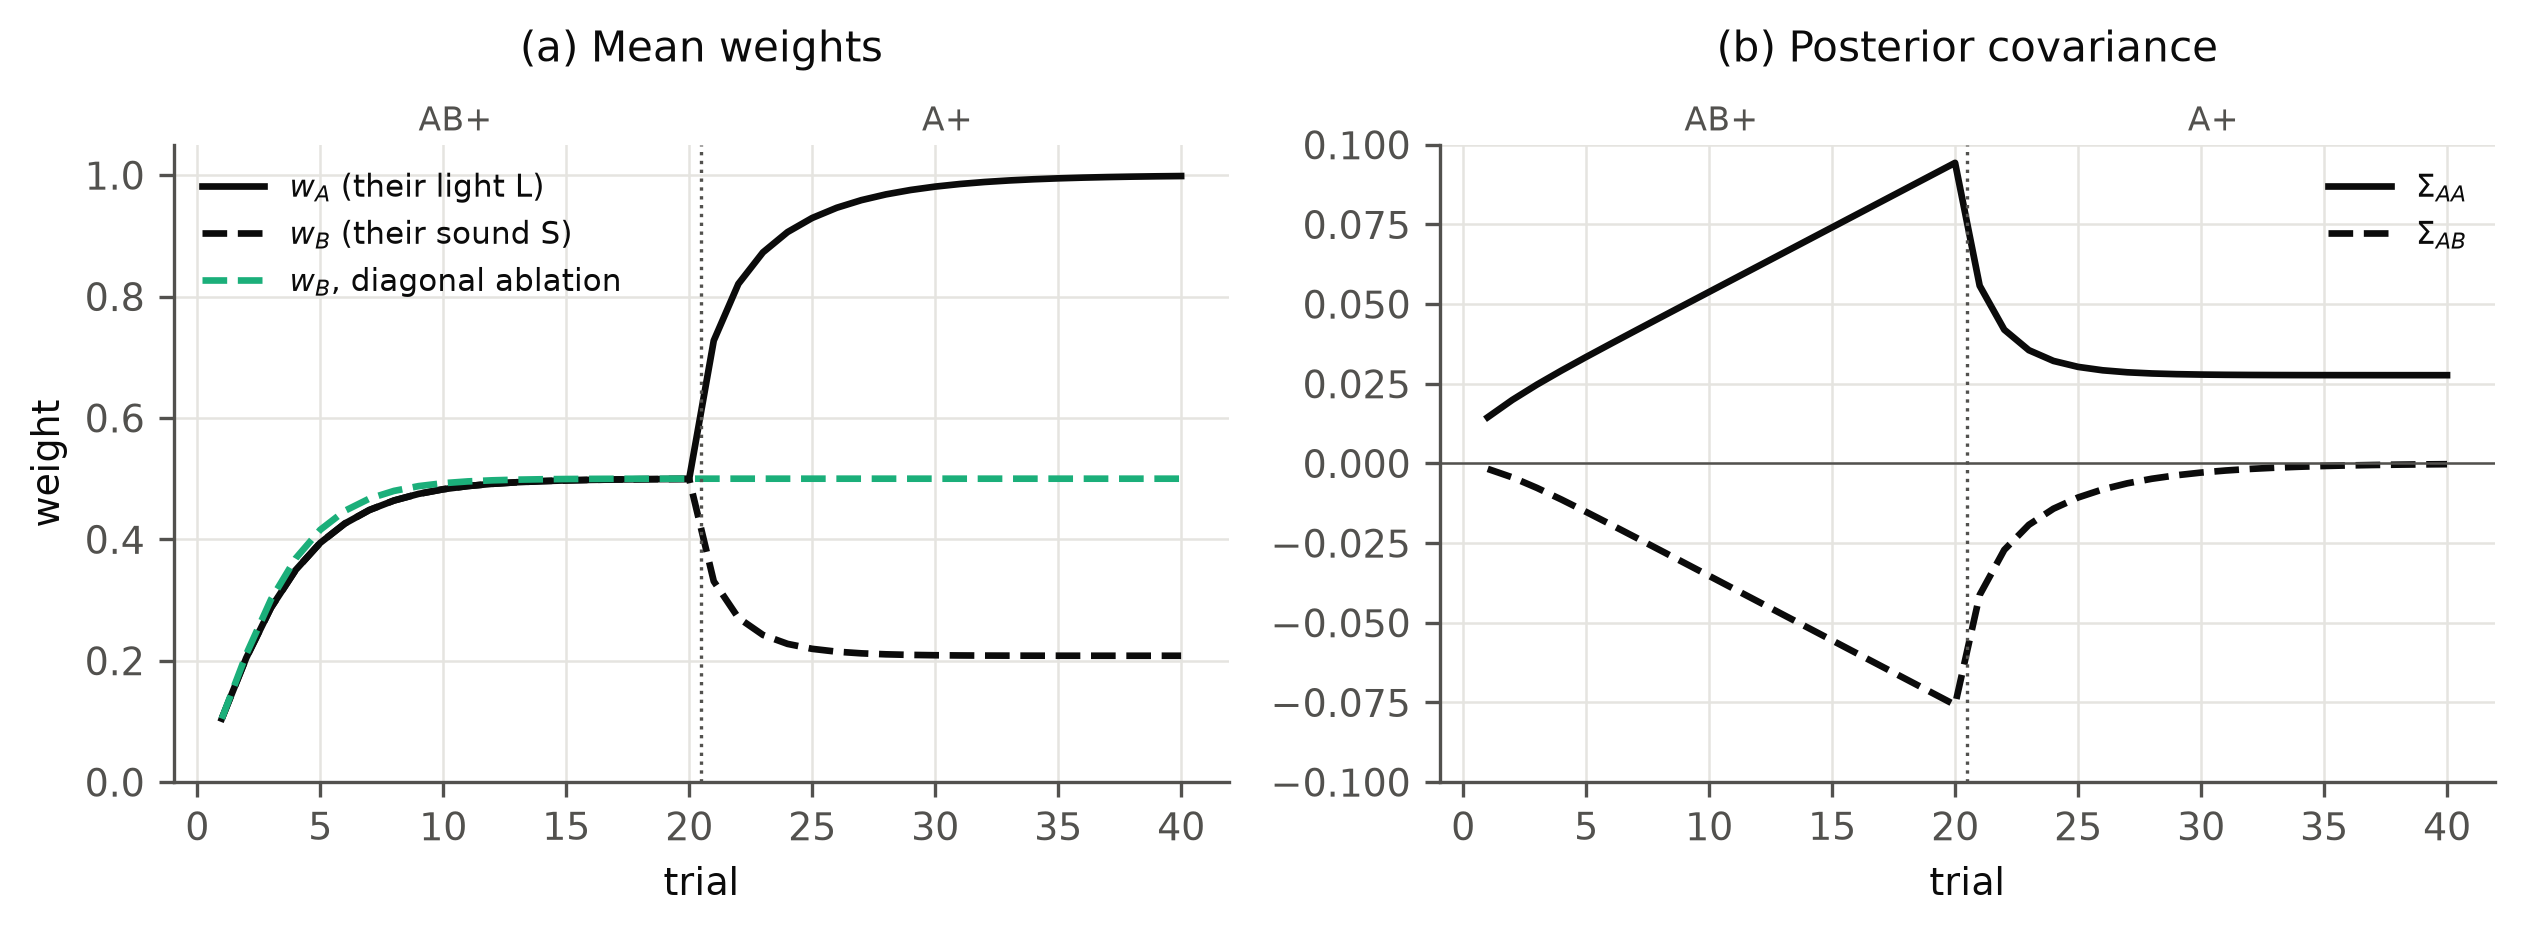
\includegraphics[width=0.72\textwidth]{fig7_dk2001_replication.png}
\caption{Reproduction of the exact Kalman-filter simulation of Dayan and Kakade
\cite{dayan2001} (their Fig.~2C--D). (a)~Weights: B is explained away once A is
trained alone; the diagonal ablation (green) shows no change. (b)~Posterior
variance of A and cross-covariance A--B.}
\label{fig:dk}
\end{figure*}

\subsection{Which Phenomena Does Each Model Produce? (H1)}
All four models showed forward blocking and overshadowing (Table~\ref{tab:effects},
Fig.~\ref{fig:rep}). Only the full Kalman learner produced backward blocking and
unovershadowing; for RW and the diagonal Kalman learner both effects were exactly
zero. Under reward noise the Kalman effects were $0.433\pm0.047$ (BB) and
$0.405\pm0.047$ (UO), positive in 20/20 seeds (Fig.~\ref{fig:eff}). H1 is
supported. Acquisition was faster for the Kalman learner (5 vs.\ 22 trials), but
this depends on the arbitrary choice $\alpha=0.1$ and is not a meaningful comparison.

\begin{table}[!t]
\centering\footnotesize
\setlength{\tabcolsep}{3.5pt}
\caption{Effect Sizes With Deterministic Rewards (Default Parameters)}
\label{tab:effects}
\begin{tabular}{lcccc}
\toprule
Model & FB & OS & BB & UO\\
\midrule
Rescorla--Wagner & 0.478 & 0.458 & 0.000 & 0.000\\
Kalman (full) & 0.498 & 0.498 & \textbf{0.419} & \textbf{0.419}\\
Kalman (diagonal) & 0.498 & 0.498 & 0.000 & 0.000\\
RW + within-compound & 0.478 & 0.458 & 0.126 & 0.126\\
\bottomrule
\end{tabular}\\[3pt]
\raggedright\scriptsize FB: forward blocking; OS: overshadowing; BB: backward
blocking; UO: unovershadowing.
\end{table}

\begin{figure*}[!t]
\centering
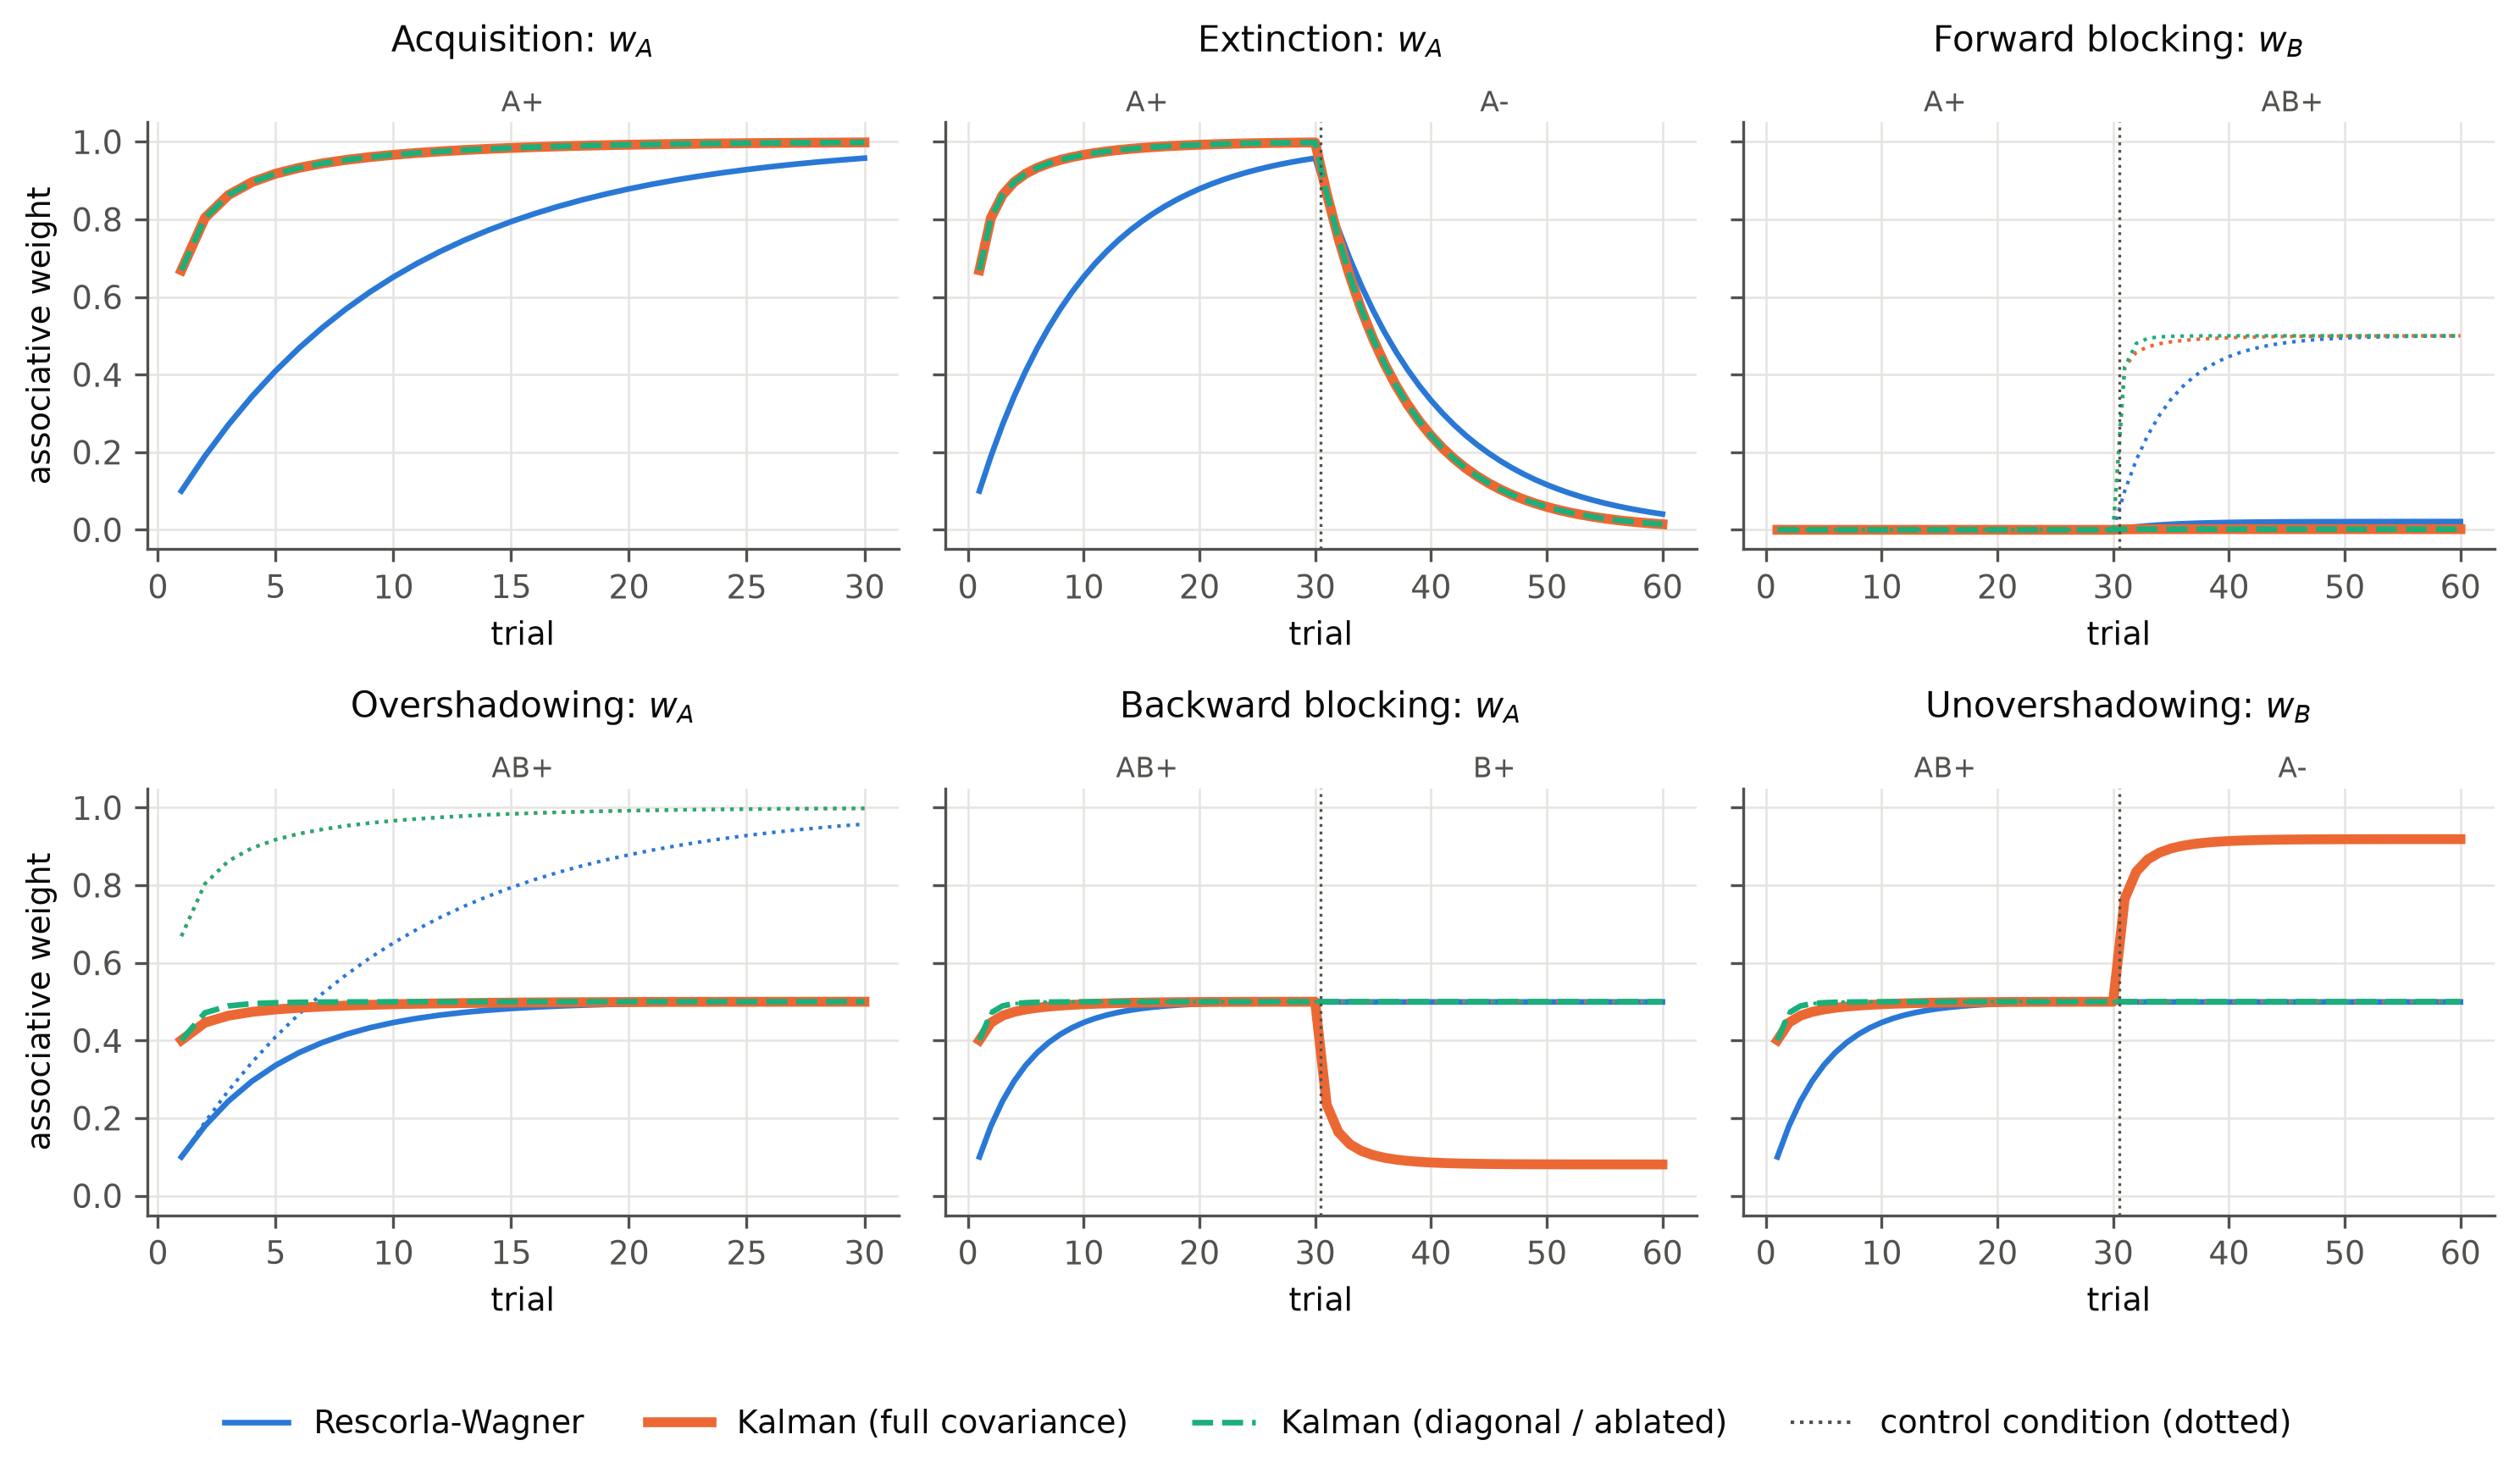
\includegraphics[width=0.85\textwidth]{fig1_replication.png}
\caption{Critical-cue weights across six paradigms. Dotted lines show control
conditions. The full Kalman learner (orange) diverges from RW (blue) and the
diagonal ablation (green, dashed) only in backward blocking and unovershadowing.}
\label{fig:rep}
\end{figure*}

\begin{figure}[!t]
\centering
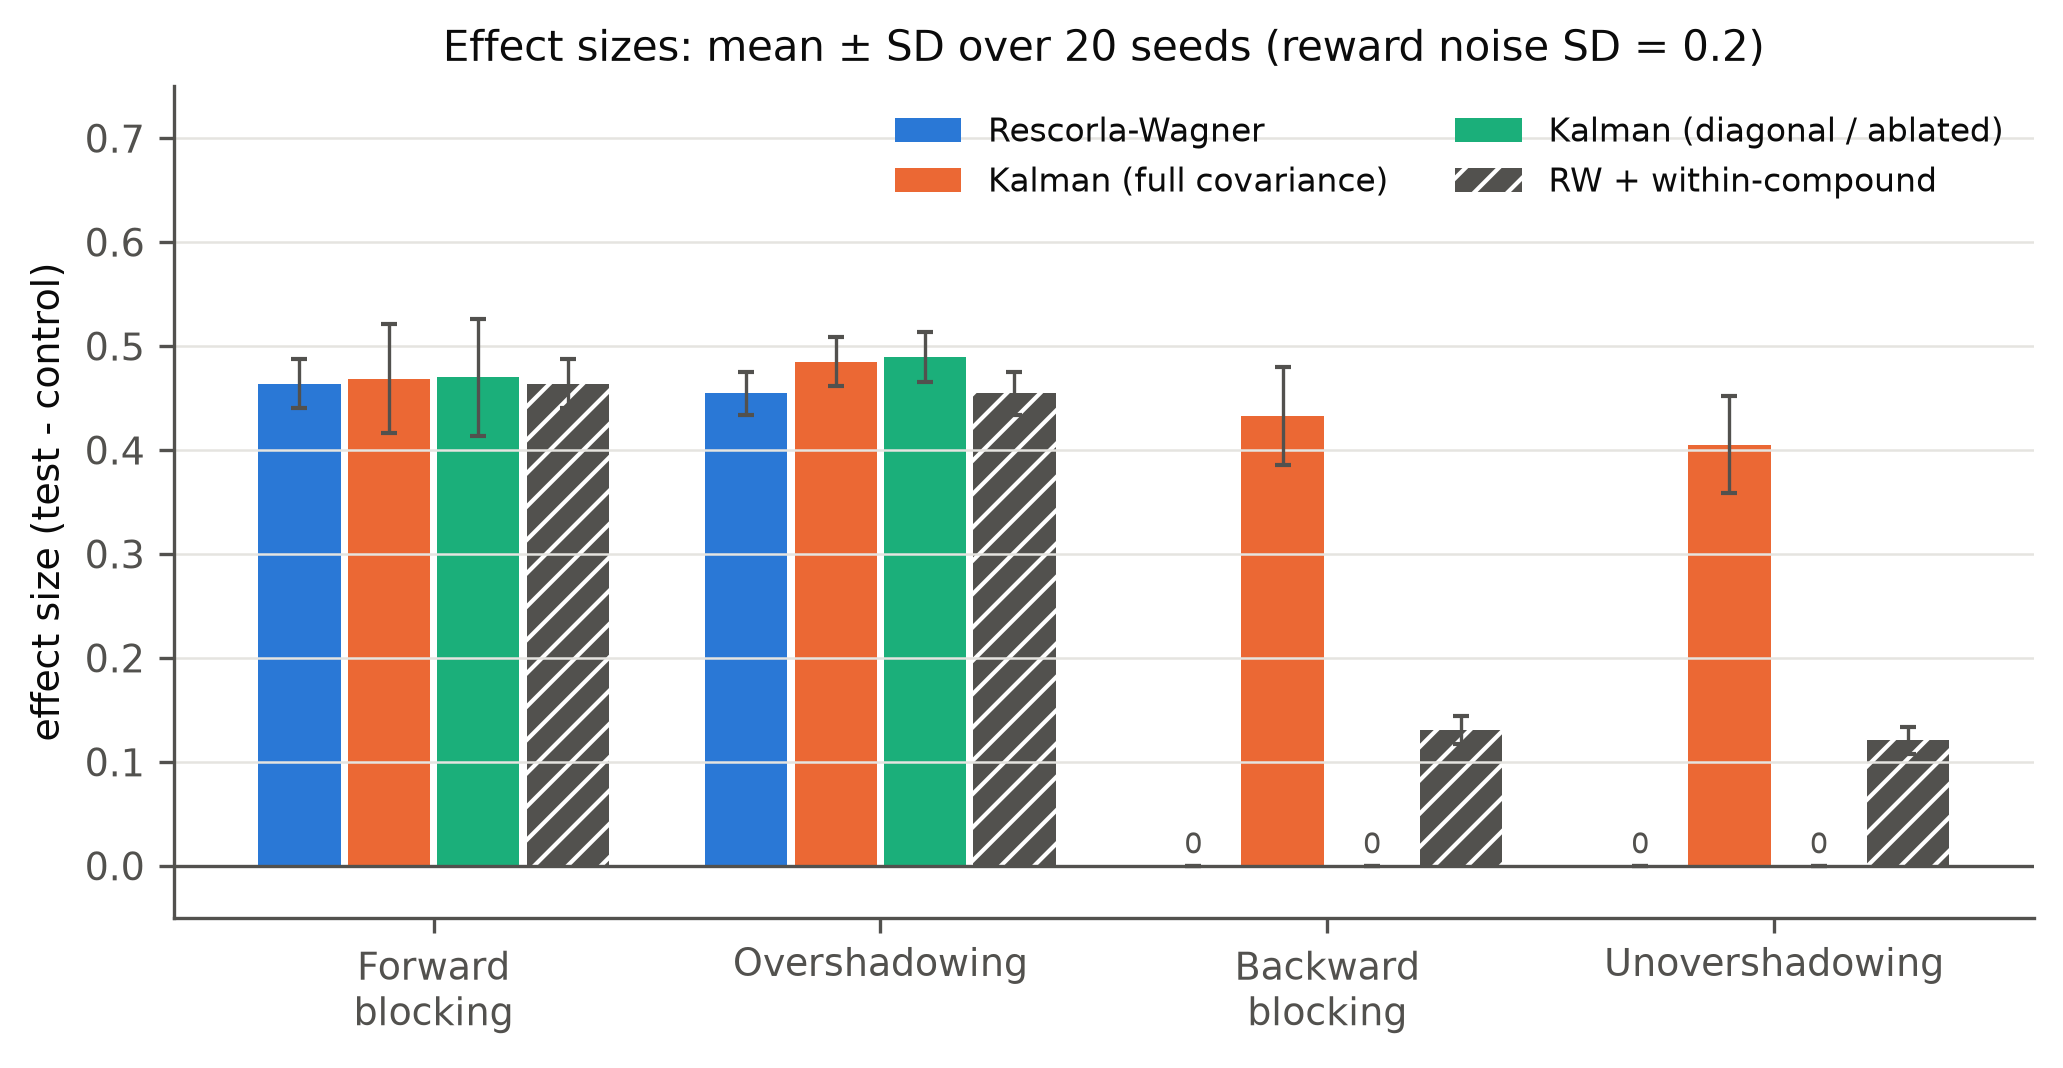
\includegraphics[width=\columnwidth]{fig2_effect_sizes.png}
\caption{Effect sizes (test $-$ control), mean $\pm$ SD over 20 reward-noise seeds.}
\label{fig:eff}
\end{figure}

\subsection{How Does Backward Blocking Arise Inside the Filter?}
Fig.~\ref{fig:mech} traces the mechanism. After 30 AB$+$ trials,
$\Sigma_{AA}=\Sigma_{BB}=0.673$ and $\Sigma_{AB}=-0.627$, a correlation of
$-0.92$. On the first B$+$ trial, $\delta=0.5$, and the gains were
$k_B=0.683/1.183=0.577$ and $k_A=-0.627/1.183=-0.530$. So $w_B$ rose to $0.79$
while the absent cue's weight $w_A$ fell from $0.50$ to $0.24$ on that single trial.
As B became well determined, $\Sigma_{AB}$ decayed to zero and the transfer stopped.

\begin{figure*}[!t]
\centering
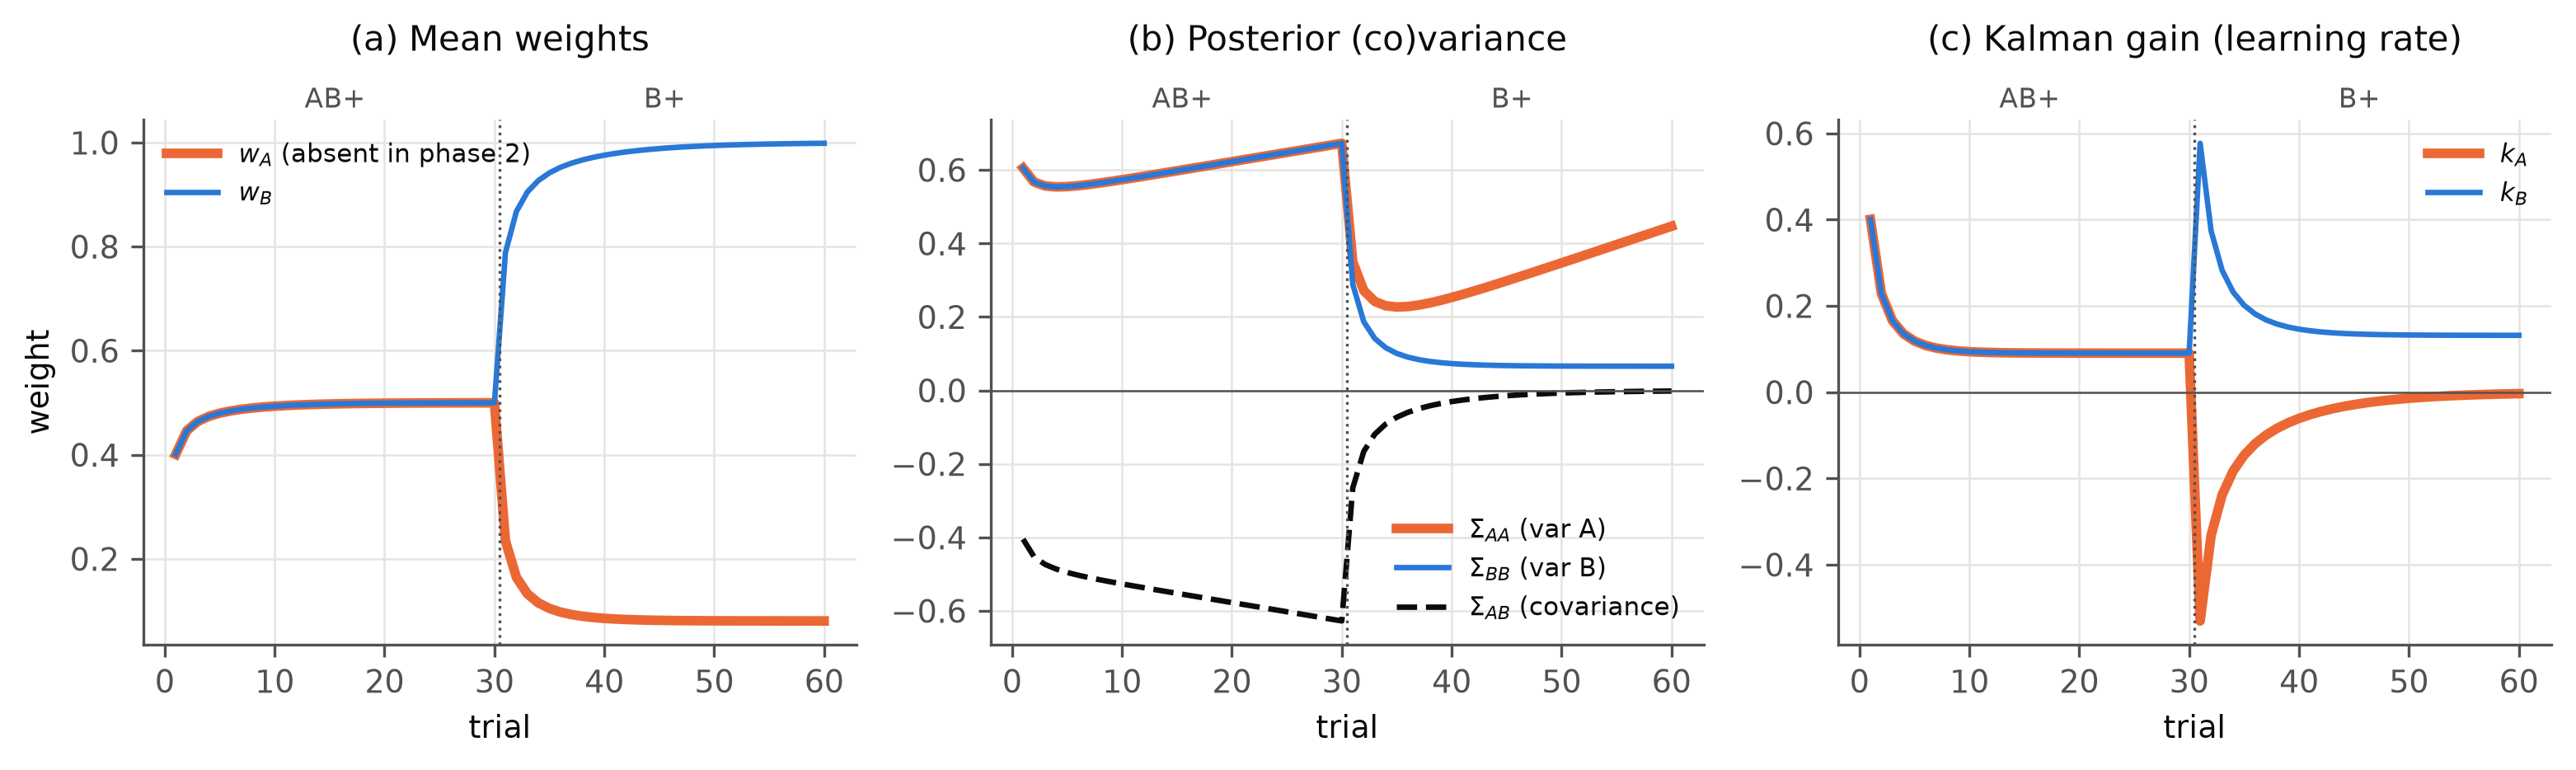
\includegraphics[width=\textwidth]{fig3_kalman_mechanism.png}
\caption{Kalman internals during backward blocking. (a)~Weights. (b)~Variances
and cross-covariance. (c)~Gains: the absent cue A receives a \emph{negative} gain
in phase 2.}
\label{fig:mech}
\end{figure*}

\subsection{How Do Process and Observation Noise Shape the Effects? (H3)}
Backward blocking was present at every point in the $10\times10$ grid
(Fig.~\ref{fig:sweep}a): $0.23$--$0.50$ after 30 B$+$ trials. Contrary to H3,
it did not require process noise. With $\tau^2 = 0$ it ranged from $0.27$
($\sigma^2=10$) to $0.50$ ($\sigma^2=0.01$). Without drift, the negative covariance
comes entirely from the prior combined with compound training. The 30-trial
measure saturates near its ceiling of $0.5$, so I also measured backward blocking
after only five B$+$ trials (Fig.~\ref{fig:sweep}b). This measure was much more
sensitive to observation noise: at $\tau^2=0$ it fell from $0.50$ to $0.10$ as
$\sigma^2$ rose, whereas at $\tau^2=1$ it stayed between $0.36$ and $0.47$.
Acquisition followed the expected pattern (Fig.~\ref{fig:sweep}c). It slowed with
$\sigma^2$ (1 to 90 trials at $\tau^2=0$) and speeded up with $\tau^2$ (at most 9
trials at $\tau^2=1$). Unovershadowing mirrored backward blocking
(range $0.20$--$0.50$).

\begin{figure*}[!t]
\centering
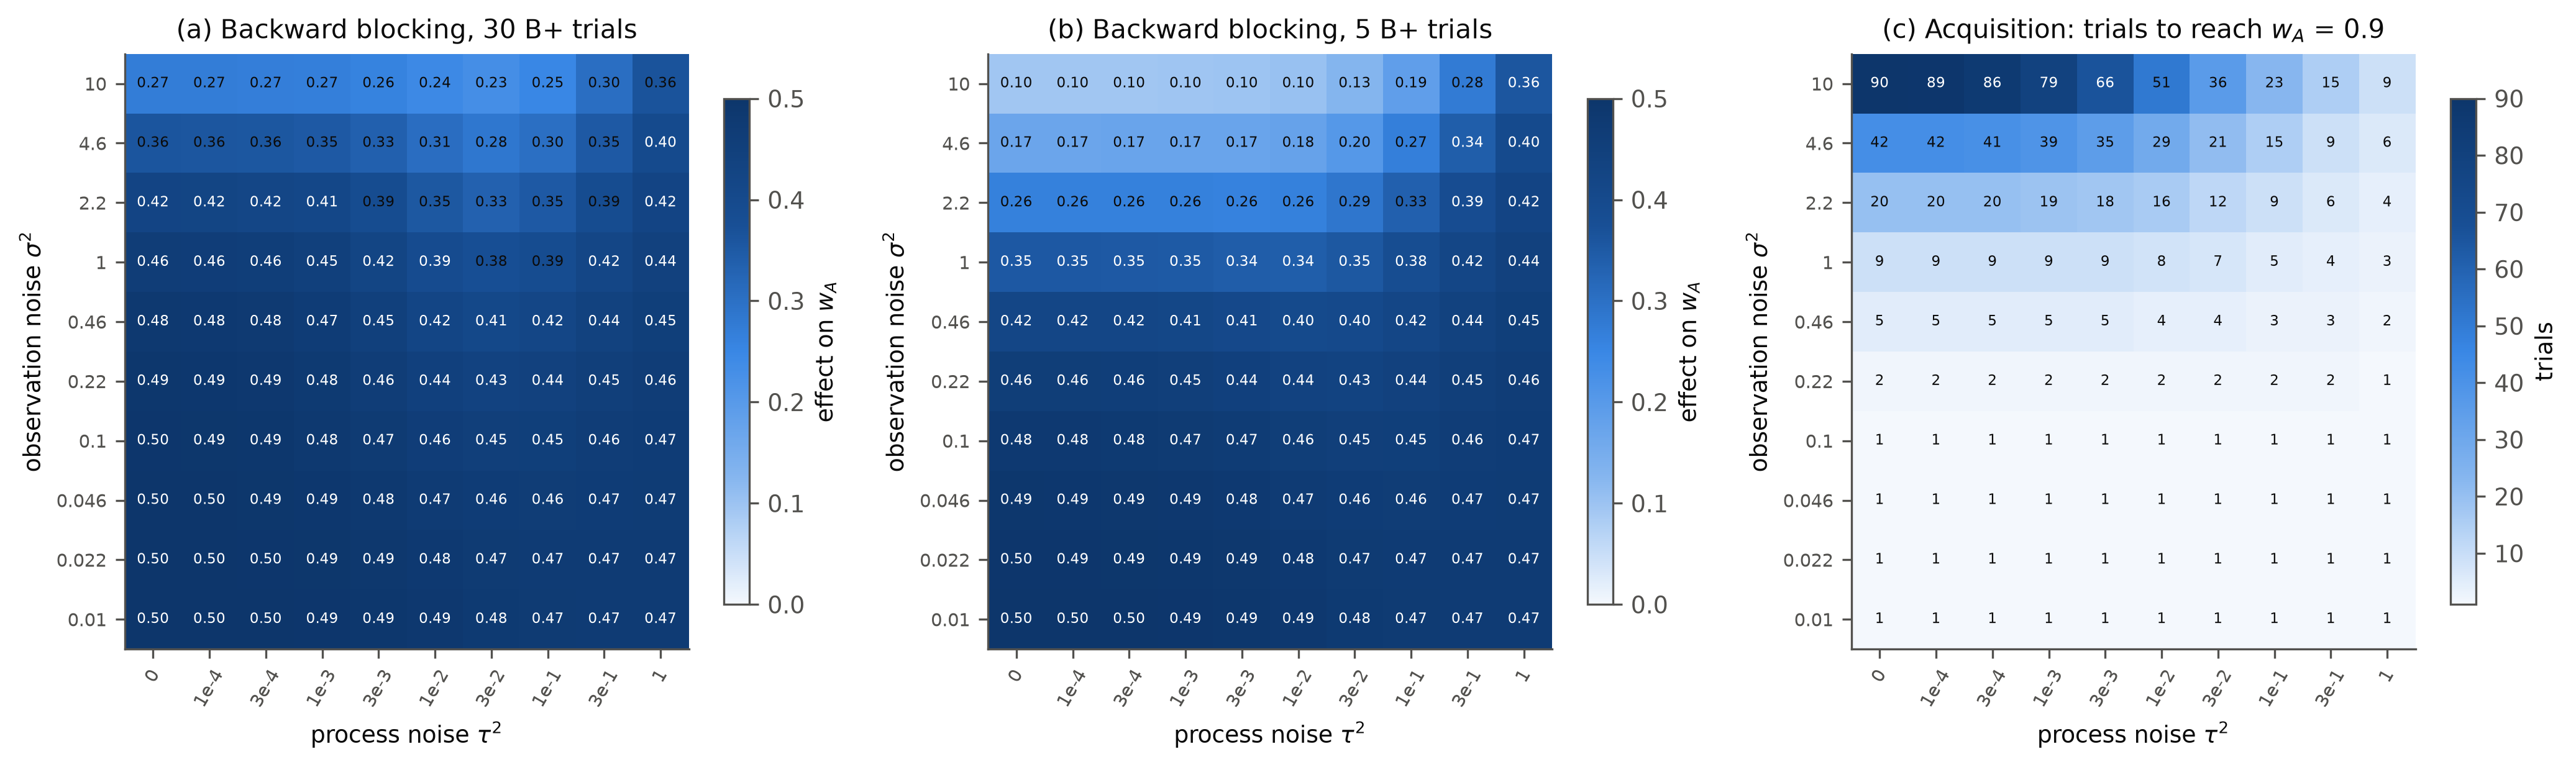
\includegraphics[width=\textwidth]{fig4_noise_sweep.png}
\caption{Noise sweep for the full Kalman learner. (a)~Backward blocking after 30
B$+$ trials. (b)~After 5 B$+$ trials. (c)~Trials to reach $w_A=0.9$ in acquisition.}
\label{fig:sweep}
\end{figure*}

The effect of $\tau^2$ on backward blocking was \emph{non-monotonic}
(Fig.~\ref{fig:abl}a). At $\sigma^2=0.5$ it was $0.48$ at $\tau^2=0$, dipped to
$0.41$ near $\tau^2\approx0.03$, and recovered to $0.45$ at $\tau^2=1$.
Table~\ref{tab:diag} suggests why. Larger $\tau^2$ makes the first B$+$ trial
more decisive ($k_A$ from $-0.49$ to $-0.90$). However, drift is added to each
cue independently during phase 2, which decorrelates A and B, so $w_A$ stops
falling earlier. With no drift, $w_A$ keeps falling to $0.016$. At intermediate
$\tau^2$ neither force dominates. I offer this as an interpretation supported by
the table, not as a formal proof.

\begin{table}[!t]
\centering\footnotesize
\setlength{\tabcolsep}{3pt}
\caption{Diagnosing the Non-Monotonic Effect of $\tau^2$ ($\sigma^2=0.5$; Test Schedule Only)}
\label{tab:diag}
\begin{tabular}{cccccc}
\toprule
 & corr$(A,B)$ & $k_A$ on & \multicolumn{3}{c}{$w_A$ after $n$ B$+$ trials}\\
\cmidrule(lr){4-6}
$\tau^2$ & entering B$+$ & first B$+$ & $n=1$ & $n=5$ & $n=30$\\
\midrule
0 & $-0.984$ & $-0.494$ & 0.247 & 0.082 & 0.016\\
0.01 & $-0.919$ & $-0.530$ & 0.235 & 0.105 & 0.081\\
0.03 & $-0.899$ & $-0.602$ & 0.199 & 0.102 & 0.094\\
0.1 & $-0.900$ & $-0.731$ & 0.135 & 0.085 & 0.084\\
1 & $-0.927$ & $-0.900$ & 0.050 & 0.046 & 0.046\\
\bottomrule
\end{tabular}
\end{table}

\subsection{Is the Cross-Cue Covariance Necessary? (H2)}
Yes. With the off-diagonal covariance removed, backward blocking and
unovershadowing were exactly zero at all 100 parameter settings, while forward
blocking remained between $0.31$ and $0.50$ (Fig.~\ref{fig:abl}a). This outcome
follows analytically from the gain equation: with diagonal $\Sig$, an absent cue's
gain is zero. The informative result is therefore the dissociation. Forward
blocking and overshadowing depend only on the shared prediction error, while the
retrospective effects depend only on the covariance. H2 is supported.

Two further properties emerged (Fig.~\ref{fig:abl}b--c). With $\tau^2>0$,
$\Sigma_{AB}$ grows without bound during compound training (to $-5.44$ after 100
trials at $\tau^2=0.1$). As a result, backward blocking keeps increasing with the
length of the AB$+$ phase ($0.29$ after 1 trial to $0.47$ after 100). With
$\tau^2=0$, both saturate within about 20 trials.

\begin{figure*}[!t]
\centering
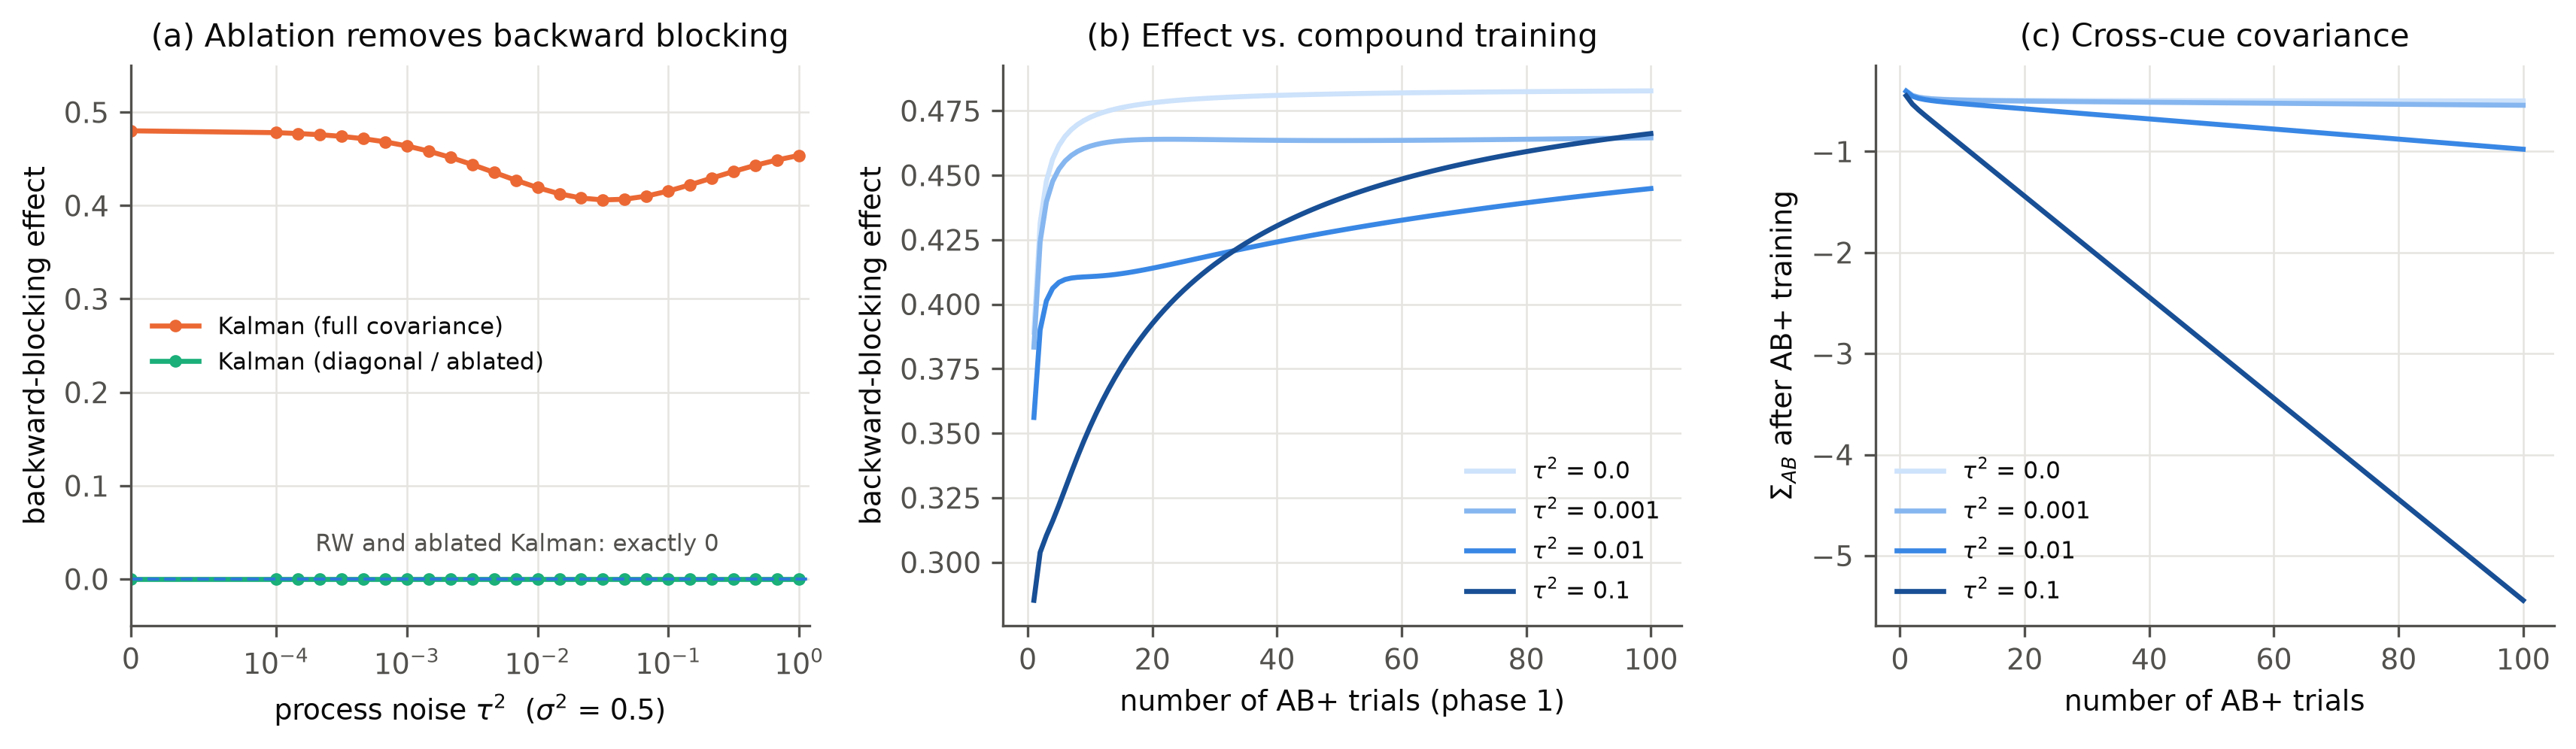
\includegraphics[width=\textwidth]{fig5_ablation.png}
\caption{(a)~Backward blocking versus $\tau^2$ for full and diagonal covariance
($\sigma^2=0.5$). (b)~Backward blocking versus number of AB$+$ trials.
(c)~Cross-covariance $\Sigma_{AB}$ during AB$+$ training.}
\label{fig:abl}
\end{figure*}

\subsection{Can a Non-Bayesian Model Produce the Same Effects?}
Yes. The within-compound RW model produced backward blocking and unovershadowing
(both $0.126$; under noise $0.131\pm0.013$ and $0.121\pm0.013$, 20/20 seeds;
Fig.~\ref{fig:alt}). The effects were weaker than the Kalman learner's, but I did
not tune its two extra parameters. The difference in size therefore does not
show that one model is better.

\begin{figure*}[!t]
\centering
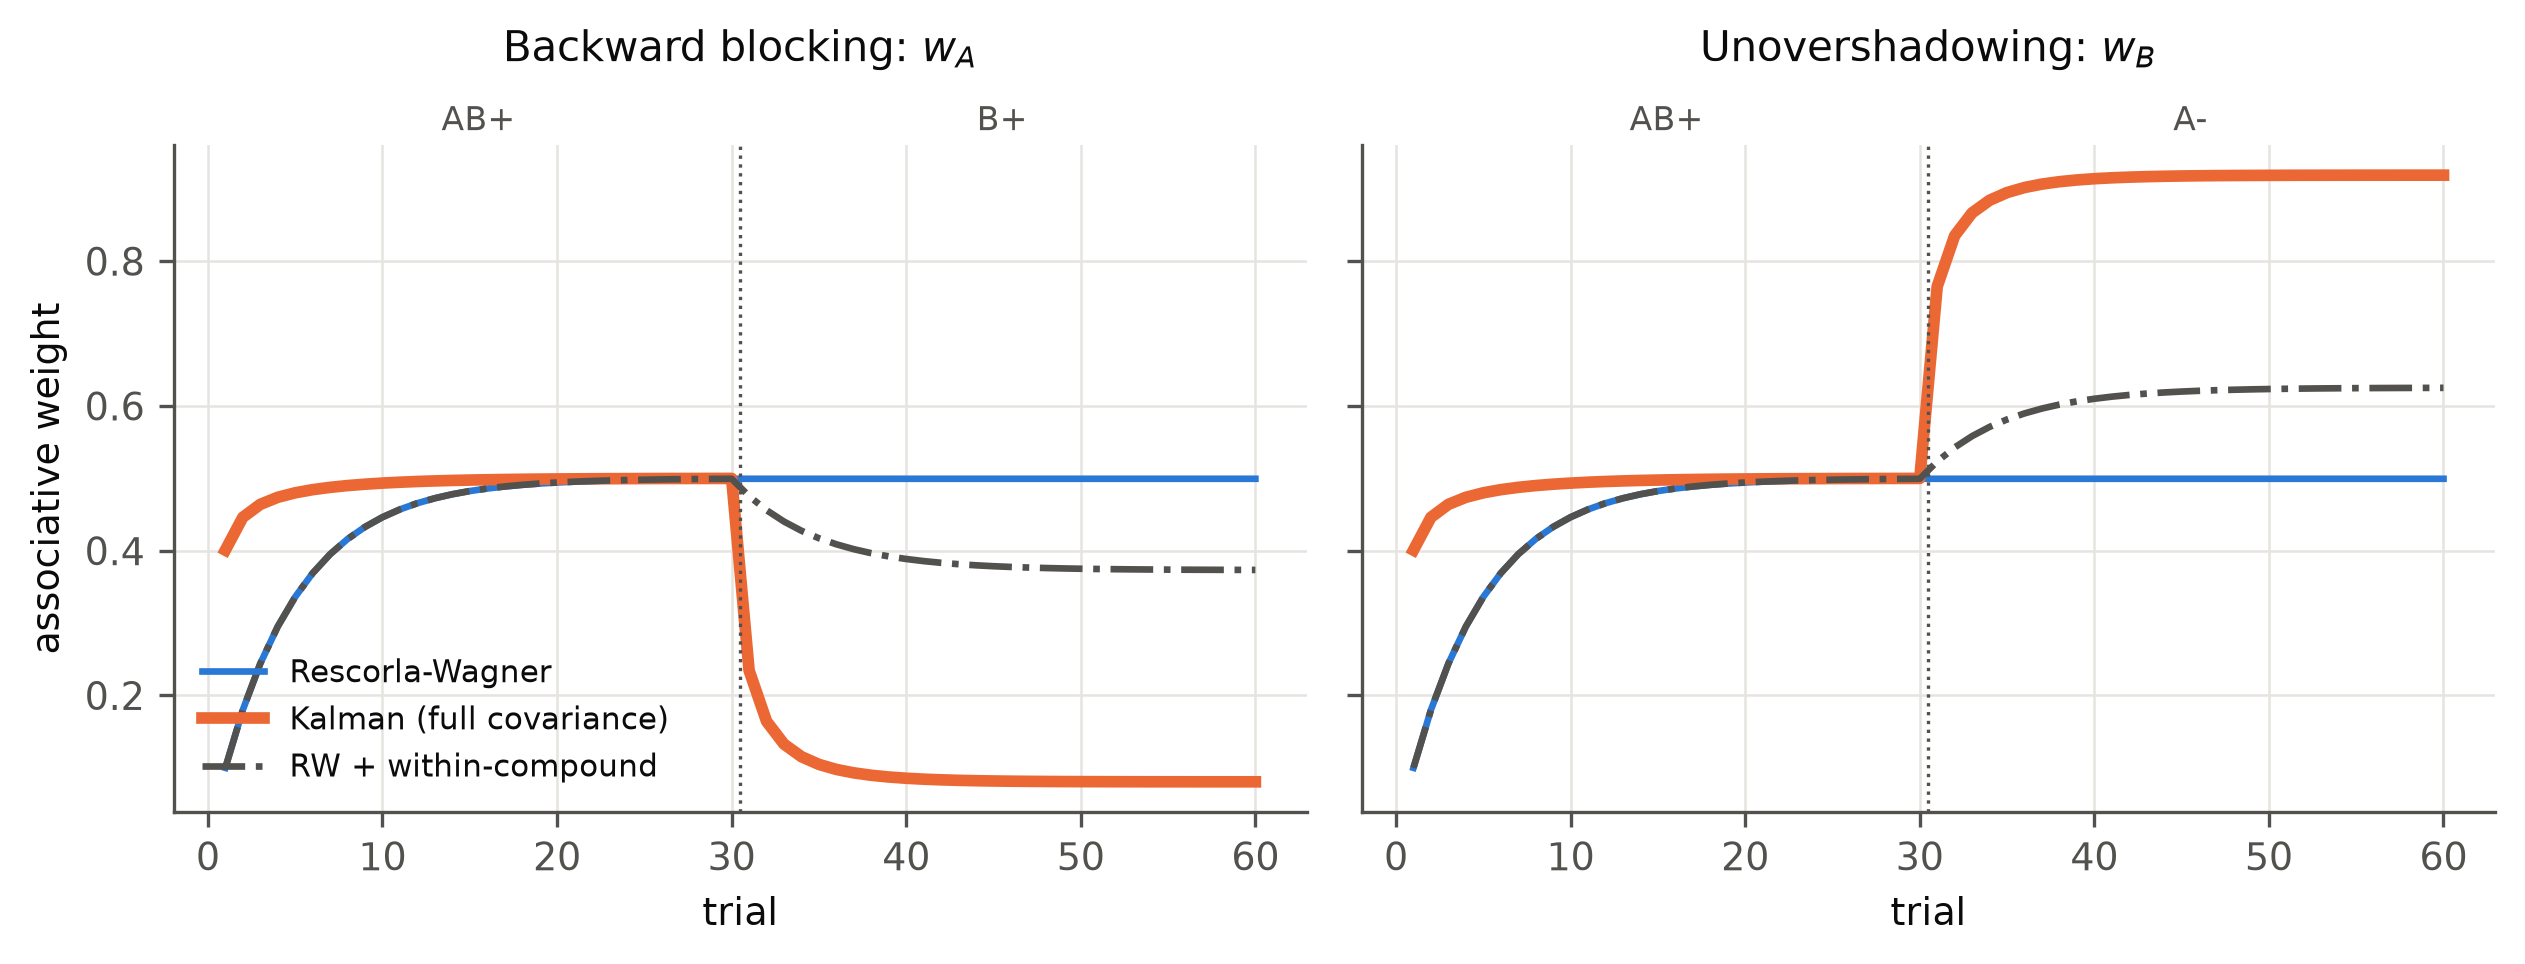
\includegraphics[width=0.72\textwidth]{fig6_alternative_model.png}
\caption{Kalman learner versus RW with within-compound associations (dash-dot).
Both revalue the absent cue; RW does not.}
\label{fig:alt}
\end{figure*}

%=====================================================================
\section{Discussion}
%=====================================================================
\subsection{Interpretation of Findings}
\subsubsection{What the Model Explains}
Unlike RW, the Kalman learner produces backward blocking and unovershadowing as
well as the standard effects. The responsible component is the off-diagonal
covariance: the learner's knowledge that its uncertainties about two cues are
linked. The diagonal model keeps adaptive, competitively shared gains, as in
\cite{dkm2000}, yet cannot revalue an absent cue. This turns the remark of Dayan
and Kakade \cite{dayan2001} about Sutton's approximation into a dissociation
across the parameter space. My expectation that drift would drive the effect (H3)
was wrong. Drift mainly controls acquisition speed and the time course of
revaluation.

\subsubsection{Where It Fails}
First, the model predicts backward blocking almost as large as forward blocking
($0.42$ vs.\ $0.50$) for all parameters I tested. In animals, backward blocking is
weaker and depends on conditions \cite{miller1996}. Only removing the covariance
altogether separates the two; Dayan and Kakade \cite{dayan2001} suggest that the
neural machinery for it may not always be available, which is equivalent to my
ablation. Second, with drift the covariance along unconstrained directions grows
without bound. This predicts ever-stronger revaluation after longer compound
training, which has not, as far as I know, been tested. Third, extinction is pure
unlearning, so the model cannot produce spontaneous recovery or renewal. Fourth,
the linear-Gaussian model cannot represent configural learning.

\subsubsection{An Alternative Explanation}
The same effects arise from RW extended with within-compound associations
\cite{vanhamme1994}, an idea also central to Wagner's SOP/AESOP framework
\cite{wagner1989}. Here A is ``retrieved'' when B is presented and, because it is
absent, it learns with a negative rate. The two accounts differ in how they treat
trial order. Without drift, the Kalman posterior depends only on the set of trials
and not on their order, so forward and backward blocking must end equally strong.
Presenting 30 A$+$ and 30 AB$+$ trials in either order left $w_B=0.016$ both
times. Drift makes forward blocking somewhat stronger than backward blocking
($w_B = 0.002$ vs.\ $0.081$ at $\tau^2=0.01$). The within-compound model builds in
a much larger asymmetry ($0.021$ vs.\ $0.373$). Data that measure \emph{how much}
weaker backward blocking is than forward blocking under matched conditions could
therefore separate the accounts, and the Kalman account would need substantial
drift to produce a large asymmetry.

\subsection{Limitations and Future Directions}
The replication of \cite{dayan2001} is qualitative, with an assumed prior. All
data are simulated, no model was fitted to behaviour, weights were read out
without a response model, and parameters were hand-chosen. The 30-trial measures
saturate (partly addressed by the 5-trial measure), and the within-compound
model is simplified. Future work could fit both models to published
trial-by-trial causal-judgement data, add a response model, test the predicted
dependence of backward blocking on compound-phase length, and compare the Kalman
learner with latent-cause models \cite{gershman2015}.

%=====================================================================
\section*{Contribution Statement}
%=====================================================================
This was an individual project, and I scoped the work to one model family with
one extension (backward blocking and unovershadowing), one ablation and one
competing model. I chose the research question and the replicate-and-extend
design, specified the models, paradigms and analyses, ran and checked all
simulations, interpreted the results, and prepared this report, the slides and
the project video. An AI assistant (Claude, by Anthropic) was used for background
research, code assistance, debugging, and implementing verification checks and
analyses. All code and results were reviewed and verified by me.

%=====================================================================
% References in IEEE style, numbered in order of first citation.
%=====================================================================
\begin{thebibliography}{99}

\bibitem{rescorla1972}
R.~A. Rescorla and A.~R. Wagner, ``A theory of Pavlovian conditioning: Variations
in the effectiveness of reinforcement and nonreinforcement,'' in \emph{Classical
Conditioning II: Current Research and Theory}, A.~H. Black and W.~F. Prokasy, Eds.
New York, NY, USA: Appleton-Century-Crofts, 1972, pp.~64--99.

\bibitem{shanks1985}
D.~R. Shanks, ``Forward and backward blocking in human contingency judgement,''
\emph{Quart. J. Exp. Psychol.}, vol.~37B, pp.~1--21, 1985.

\bibitem{matzel1985}
L.~D. Matzel, T.~R. Schachtman, and R.~R. Miller, ``Recovery of an overshadowed
association achieved by extinction of the overshadowing stimulus,''
\emph{Learn. Motiv.}, vol.~16, no.~4, pp.~398--412, 1985.

\bibitem{dayan2001}
P.~Dayan and S.~Kakade, ``Explaining away in weight space,'' in \emph{Advances in
Neural Information Processing Systems 13}. Cambridge, MA, USA: MIT Press, 2001,
pp.~451--457.

\bibitem{sutton1992}
R.~S. Sutton, ``Gain adaptation beats least squares?'' in \emph{Proc. 7th Yale
Workshop on Adaptive and Learning Systems}, New Haven, CT, USA, 1992, pp.~161--166.

\bibitem{dkm2000}
P.~Dayan, S.~Kakade, and P.~R. Montague, ``Learning and selective attention,''
\emph{Nature Neurosci.}, vol.~3, suppl., pp.~1218--1223, 2000,
doi: 10.1038/81504.

\bibitem{pearce1980}
J.~M. Pearce and G.~Hall, ``A model for Pavlovian learning: Variations in the
effectiveness of conditioned but not of unconditioned stimuli,''
\emph{Psychol. Rev.}, vol.~87, no.~6, pp.~532--552, 1980.

\bibitem{kakade2002}
S.~Kakade and P.~Dayan, ``Acquisition and extinction in autoshaping,''
\emph{Psychol. Rev.}, vol.~109, no.~3, pp.~533--544, 2002.

\bibitem{kruschke2008}
J.~K. Kruschke, ``Bayesian approaches to associative learning: From passive to
active learning,'' \emph{Learn. Behav.}, vol.~36, no.~3, pp.~210--226, 2008,
doi: 10.3758/LB.36.3.210.

\bibitem{gershman2015}
S.~J. Gershman, ``A unifying probabilistic view of associative learning,''
\emph{PLoS Comput. Biol.}, vol.~11, no.~11, Art.~no.~e1004567, 2015,
doi: 10.1371/journal.pcbi.1004567.

\bibitem{vanhamme1994}
L.~J. Van~Hamme and E.~A. Wasserman, ``Cue competition in causality judgments: The
role of nonpresentation of compound stimulus elements,'' \emph{Learn. Motiv.},
vol.~25, no.~2, pp.~127--151, 1994.

\bibitem{wagner1989}
A.~R. Wagner and S.~E. Brandon, ``Evolution of a structured connectionist model of
Pavlovian conditioning (AESOP),'' in \emph{Contemporary Learning Theories},
S.~B. Klein and R.~R. Mowrer, Eds. Hillsdale, NJ, USA: Erlbaum, 1989, pp.~149--189.

\bibitem{miller1996}
R.~R. Miller and H.~Matute, ``Biological significance in forward and backward
blocking: Resolution of a discrepancy between animal conditioning and human causal
judgment,'' \emph{J. Exp. Psychol.: Gen.}, vol.~125, no.~4, pp.~370--386, 1996.

\end{thebibliography}

\end{document}
